\subsubsection{结合相同场景的移动轨迹分析耗时差异}\label{sec:q3-13}

为了将费用差异对应到具体行动，图\ref{fig:q23-6}选取首版基线用时最接近256局中位数的场景800035；
选择仅依据基线，不依据其他方法的输赢。
四种方法使用相同的源位置、接收半径与噪声场，全部清除11个源。
在此例中PPO用时2943.02 s，短于状态搜索的3118.22 s，与总体均值的排序不同。
这说明代表性轨迹用于解释行为差异，不能替代全部场景上的统计判断。

状态搜索和PPO采用了不同的清除顺序与测点。
PPO在该例移动耗时2205.02 s、测量116次；
状态搜索移动耗时2311.22 s、测量127次。
两项费用均有降低，因而共同解释本例PPO的优势。
轨迹中的源坐标只在策略终止后用于展示，规划时不使用这些真值。

\begin{figure}[!htbp]
\centering
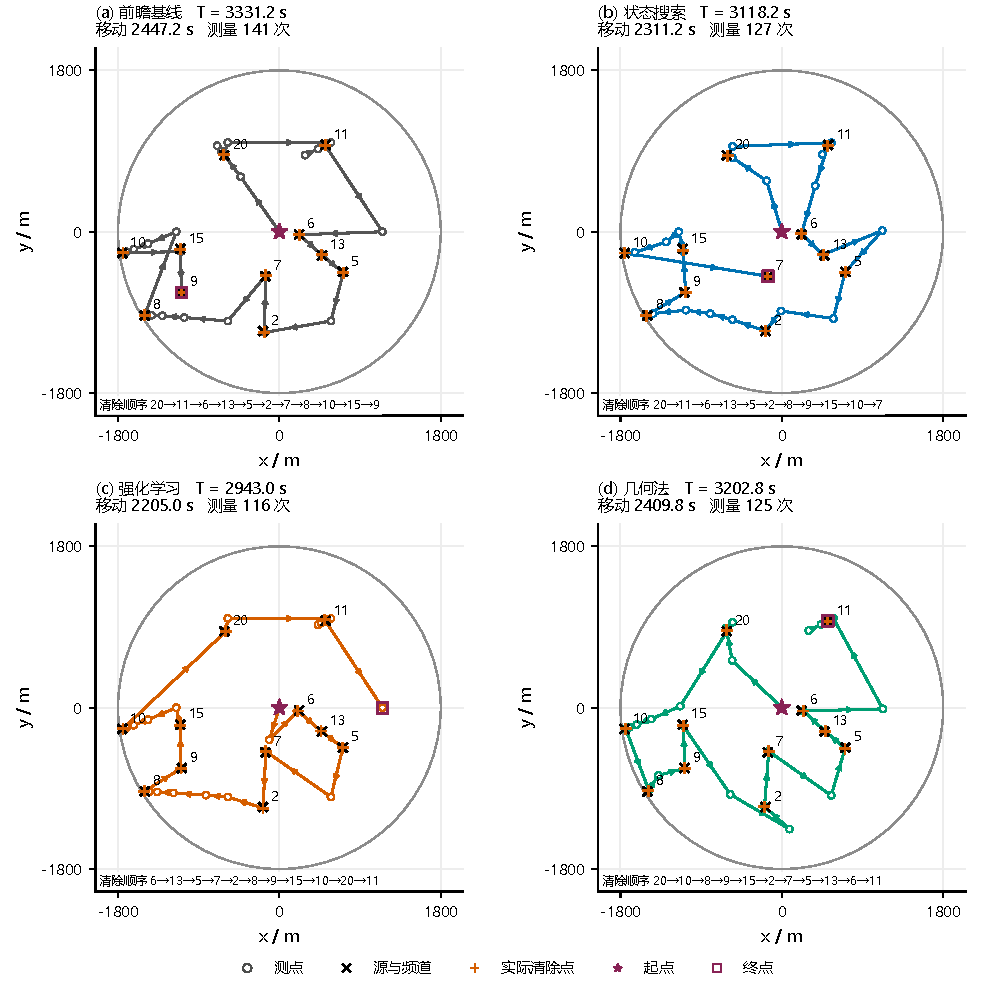
\includegraphics[width=\linewidth,height=\textheight,keepaspectratio,alt={基线中位耗时附近场景800035的四方法真实轨迹。统一坐标比例，箭头表示移动方向，源旁数字为频道，面板底部列出实际清除顺序。同坐标多次测量合并显示位置，但测量次数保留原始计数。}]{figures/fig06_trajectory_median.pdf}
\caption{基线中位耗时附近场景800035的四方法真实轨迹。统一坐标比例，箭头表示移动方向，源旁数字为频道，面板底部列出实际清除顺序。同坐标多次测量合并显示位置，但测量次数保留原始计数。}
\label{fig:q23-6}
\end{figure}

为展示方法的边界，附录还给出各方法相对基线退化最大的案例。
状态搜索在800015场景中增加152.08 s移动费用，虽少用25 s测量和2 s换频，最终仍多用125.08 s；
PPO在800081场景中多用340.45 s移动、20 s测量和5 s换频，最终多用365.45 s。
这些事后选择的反例揭示了长距离折返的代价，不用于估计其总体发生频率，也不据此声称已经识别出网络内部决策的因果原因。

\subsubsection{分析多源搜索效果并说明适用条件}\label{sec:q3-14}

现有结果支持在本题静止、全向、有限频道且存在可靠几何约束的条件下，以结构化规划作为有效主方案。
状态压缩合并当前任务访问顺序，主动定位控制单源信息成本，静默证书删去可证明冗余的查询，覆盖约束负责完整发现。
主实验中这一组合取得较低平均任务用时；
后期PPO接近状态搜索，则表明学习调度仍具有竞争力。

这种优势不能归结为``固定点可以普遍代替强化学习''。
主状态搜索已允许连续移动覆盖站，PPO也依赖人工候选；
二者同时利用了题目结构。
更大的状态表示、更充分的训练、不同源分布或移动源环境仍可能改变结论。
有限任务模型的最优性、连续在线策略的最优性和官方演练的成功记录属于不同层次，本稿只在各自证据范围内提出判断。

\FloatBarrier


